\documentclass[10pt]{article}
\usepackage[polish]{babel}
\usepackage[utf8]{inputenc}
\usepackage[T1]{fontenc}
\usepackage{amsmath}
\usepackage{amsfonts}
\usepackage{amssymb}
\usepackage[version=4]{mhchem}
\usepackage{stmaryrd}
\usepackage{graphicx}
\usepackage[export]{adjustbox}
\graphicspath{ {./images/} }

\title{VII Konkurs matematyczny St@ś }

\author{}
\date{}


\begin{document}
\maketitle
XIV LO im. Stanisława Staszica\\
28 maja 2007 roku

\section*{klasa VI}
Na rozwiazanie poniższych zadań masz 90 minut. Kolejność rozwiazywania tych zadań jest dowolna. Wszystkie zadania sa jednakowo punktowane. Maksymalna liczbę punktów może uzyskać jedynie petne rozwiqzanie, z uzasadnieniem i odpowiedziq.\\
Używanie korektora i korzystanie z kalkulatora jest niedozwolone.

\begin{enumerate}
  \item Rolnik zebrał 240 ton zboża. Pierwszego dnia sprzedał \(\frac{3}{5}\) zbiorów, drugiego dnia \(\frac{1}{6}\) reszty. Ile zboża zostało rolnikowi po drugiej sprzedaży?
  \item Trzy kolejne liczby trzycyfrowe zapisano obok siebie bez odstępów, otrzymując liczbę dziewięciocyfrową podzielną przez 4 i 25. Znajdź tę liczbę, wiedząc, że w jej zapisie występują jedynie trzy różne cyfry.
  \item Oblicz objętość prostopadłościanu wiedząc, że jeśli byśmy zwiększyli o 1 cm :\\
(a) jedynie długość jego podstawy, to objętość wzrosłaby o \(20 \mathrm{~cm}^{3}\).\\
(b) jedynie szerokość jego podstawy, to objętość wzrosłaby o \(50 \mathrm{~cm}^{3}\).\\
(c) jedynie jego wysokość, to objętość wzrosłaby o \(10 \mathrm{~cm}^{3}\).
  \item Dany jest równoległobok \(A B C D\) o polu równym \(20 \mathrm{~cm}^{2}\). Punkt \(P\) znajduje się we wnętrzu tego równoległoboku. Oblicz sumę pól trójkątów \(A B P\) i \(C D P\).
  \item Uzupełnij przedstawiony poniżej diagram tak, aby każda liczba znajdująca się wyżej była dzielnikiem wszystkich liczb znajdujących się niżej.\\
W każde pole należy wpisać po jednej cyfrze. Powstaną w ten sposób cztery liczby: na górze liczba jednocyfrowa, poniżej dwu i trzycyfrowa, a na samym dole czterocyfrowa.\\
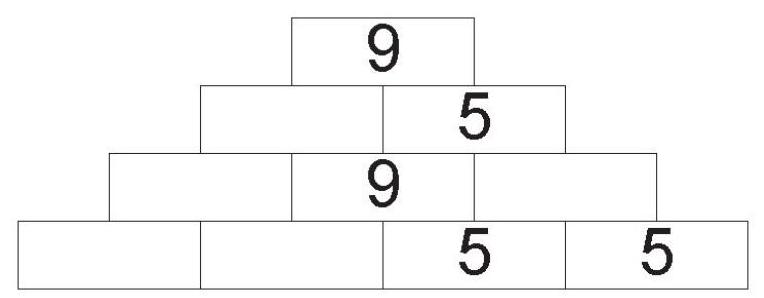
\includegraphics[max width=\textwidth, center]{2024_11_21_4666129bb05a0ea31c95g-1}
\end{enumerate}

\end{document}